\documentclass{article}
\usepackage{amsmath, amssymb, array, enumerate, tikz, multicol, hyperref, sfmath, pgfplots, tcolorbox}
\pgfplotsset{compat = newest}
\renewcommand{\familydefault}{\sfdefault}
\usepackage[top = 0.5in, bottom=0.5in, right = 1.25in, left = 1.25in]{geometry}
\tikzset{>=stealth}
\pagestyle{empty}
\raggedright

\newcounter{example}[section]
\newenvironment{example}[1][]{\refstepcounter{example}\par\medskip
   {\color{red}\textbf{Example~\theexample. #1}}}{\medskip}

\begin{document}

\section*{Factoring \pmb{$ax^2 + bx + c$}}

\begin{tcolorbox}[colframe=orange!70!white, coltitle=black, title=\textbf{Summary}]
\begin{enumerate}
    \item Always look for a greatest common factor (GCF) to factor out \emph{first}.
    \item We will use the $ac$-method of factoring with grid
\end{enumerate}
\end{tcolorbox}
\bigskip 

Recall for multiplying $(2x + 3)(7x - 1)$:  \newline\\
\begin{center}
    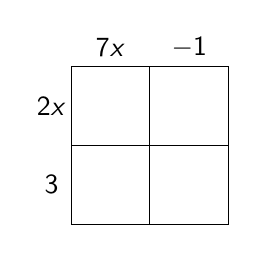
\begin{tikzpicture}
    \draw (0,0) grid (2,2);
    \node at (-0.25,1.5) {$2x$};
    \node at (-0.25,0.5) {3};
    \node at (0.5,2.25) {$7x$};
    \node at (1.5,2.25) {$-1$};
    \end{tikzpicture}
\end{center}
\bigskip 

\subsection*{The $\pmb{ac}$-Method of Factoring $\pmb{ax^2 + bx + c}$}

\begin{enumerate}
    \item Check for a GCF first. Factor out if applicable.
    \item Multiply the values of $a$ and $c$.
    \item Find 2 numbers that
    \begin{itemize}
        \item Multiply to make the value of $ac$ AND
        \item Add to make the value of $b$.
    \end{itemize}
    \item \emph{Note:} Factor out a negative when applicable.
\end{enumerate}
\vspace{0.25in} 

For instance, to factor $5x^2 - 14x + 8$: \newline 

\begin{minipage}{0.4\textwidth}
\begin{enumerate}
    \item Multiply 5 and 8 to get 40.
    \item Find 2 numbers that
    \begin{itemize}
        \item Multiply to make 40 AND
        \item Add to make $-14$
    \end{itemize}
\end{enumerate}
\end{minipage}
\hspace{1in}
\begin{minipage}{0.3\textwidth}
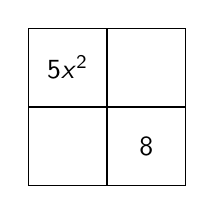
\begin{tikzpicture}
\draw (0,0) grid (2,2);
\node at (0.5,1.5) {$5x^2$};
\node at (1.5,0.5) {$8$};
\end{tikzpicture}
\end{minipage}

\vspace{0.5in} 

% One method to factoring expressions like $5x^2 - 14x + 8$ is to guess-and-check. \newline\\

% This is fine, but can take a while and get frustrating. \vspace{1in}

% Another way to approach this problem is to transform it so the coefficient of squared term is 1, \newline like in the previous section's notes. \vspace{1in}

% \subsubsection*{Transforming $\mathbf{ax^2 + bx + c}$} 

% \begin{center}
% \setlength{\extrarowheight}{20pt}
% \begin{tabular}{c|c}
%     $\mathbf{ax^2 + bx + c}$ & \textbf{Example} $\mathbf{(5x^2-14x+8)}$ \\ \hline 
%     1. Find the product $a \cdot c$ & $5 \times 8 = 40$ \\[20pt]
%     2. Rewrite as $x^2 + bx + ac$ & $x^2 - 14x + 40$ \\[20pt]
%     3. Factor that like before  &   $(x-10)(x-4)$ \\[20pt]
%     4. Transform back by dividing the numbers & $\left(x - \frac{10}{5}\right)\left(x - \frac{4}{5}\right)$ \\
%      by $a = 5$ and simplify & $(x-2)\left(x-\frac{4}{5}\right)$ \\[20pt]
%     5. Slide any denominators in front of that $x$ & $(x-2)(5x-4)$ \\[20pt]
% \end{tabular}
% \end{center}

% \newpage

\begin{example}
Factor each completely. Don't forget to check for a GCF first.
\begin{enumerate}[(a)]
\begin{multicols}{2}
    \item $3x^2-20x+28$  
    \item $2x^2-9x-35$  
\end{multicols}
\vfill 
\newpage 
\begin{multicols}{2}
    \item $3x^2-13x+4$   
    \item $3x^2+10x-8$  
\end{multicols}
\vfill 
\begin{multicols}{2}
    \item $12x^2-5x-2$  
    \item $8x^2-22x+5$ 
\end{multicols}
\vfill 
\begin{multicols}{2}
    \item $8x^6-10x^5-3x^4$ 
    \item $6x^6+19x^5-7x^4$ 
\end{multicols}
\end{enumerate}
\vfill 
\end{example}




\end{document}
